\chapter{User Factor Adaptation}
\label{chp:user}

The previous Chapter~\ref{chp:temporality} has examined language shifts and presented two temporality adaptation approaches for the document classification task. 
It has shown the effectiveness of domain adaptation with the document metadata, time.

In this chapter, we 

\section{Introduction}
% demographic factors exist in text documents
Different demographic groups can show substantial linguistic variations, especially in online data~\cite{goel2016social,johannsen2015cross}. 
%Such demographic factors have significant impacts on language use in people's word expression~\cite{goel2016social}, syntax~\cite{johannsen2015cross}, etc. 
These variations can affect natural language processing models such as sentiment classifiers.
For example, researchers found that women were more likely to use the word \textit{weakness} in a positive way, while men were more likely to use the word in a negative expression~\cite{volkova2013exploring}.

Models for text classification,
the automatic categorization of documents into categories, 
typically ignore attributes about the authors of the text.
With the growing amount of text generated by users online, whose personal characteristics are highly variable,
there has been increased attention to how user demographics are associated with the text they write.
Promising recent studies have shown that incorporating demographic factors can improve text classification~\cite{volkova2013exploring,hovy2015demographic,yang2017overcoming, li2018towards}. 
\cite{lynn2017human} refer to this idea as {\em user factor adaptation}
and proposed to treat this as a domain adaptation problem in which demographic attributes constitute different domains.
We extend this line of work in a number of ways:

\begin{itemize}
\item We assemble and publish new datasets containing four demographic factors: gender, age, country, and US region. The demographic attributes are carefully inferred from profile information that is separate from the text data.
%Our data could be used for tasks beyond this work, such as the study of algorithmic bias.
\item We experiment with neural domain adaptation models~\cite{ganin2016domain}, which may provide better performance than the simpler models used in prior work on user factor adaptation.
We also propose a new model using a multitask framework with adversarial training.
\item Our approach requires demographic attributes at training time but not at test time: we learn a single representation to be invariant to demographic changes.
This approach thus requires fewer resources than prior work.
%which is important since demographic attributes are often unavailable.
\end{itemize}

In this study, we treat adapting across the demographic factors as a domain work problem, in which we consider each demographic factor as a domain. We focus on four different demographic factors (gender, age, country, region) in four English-language social media datasets (Twitter, Amazon reviews, Yelp hotel reviews, and Yelp restaurant reviews), which contain text authored by a diversity of demographic groups.

%In this study, we treat modeling the demographic factors as a domain adaptation question, which we consider each demographic factor as a domain. We focus on four different demographic factors, gender, age, country, region, on four English-language social media datasets, Twitter, Amazon, Yelp hotel and restaurant reviews, which usually own diverse demographic communities. Particularly, we examine and investigate the following two questions:
%
%\begin{itemize}
%    \item Does language show demographic variations in social media data?
%    \item How to model demographic variations in the process of text classification?
%\end{itemize}
%

We first conduct an exploratory analysis of how different demographic variables are associated with documents and document labels (Section~\ref{sec:exploratory}).
%To address the questions, we first qualitatively explore and compare linguistic patterns on topic distributions across four different demographic factors, gender, age, country, region. We build machine learning classifiers on the domain attributes and evaluate how predictable of language could help categorize the demographic identities. 
We then describe a neural model for the task of document classification that adapts to demographic factors using a multitask learning framework (Section~\ref{sec:model}). Specifically, the model is trained to predict the values of the demographic attributes from the text in addition to predicting the document label. 
%we treat the training process as  \textit{K + 1} prediction tasks, which refers to the label prediction as well as the K demographic domain tasks. For example, the gender domain task predicts if a female or male user generates the text. 
Experiments on four social media datasets show that user factor adaptation is important for document classification, and that the proposed model works well compared to alternative domain adaptation approaches (Section~\ref{sec:experiments}).




\section{Related Work}

\paragraph{Domain adaptation} tries aligning source with related target distributions to obtain more generalized feature representations and classifiers. For the text classification task, there are two conventional methods, feature augmentations~\cite{daume2007frustratingly, blitzer2006domain, huang2018examining} and domain adversarial training~\cite{ganin2016domain, chen2016adversarial, liu2017adversarial}. However, one issue with the proposed methods is they did not consider the user demographic factors, which show strong variations among social media documents. Additionally, most of the adaptation only work on two different domains, but the demographic factors have more complex domains and divergent differences between domains.

\paragraph{User factor adaptation} integrates demographic factors into the machine learning classifiers. The demographic factors usually refer to the attributes of users, such as gender, age, geographic location, etc. Online generated user texts show demographic variations in the linguistic styles, and the linguistic style differences could be used for the use factor prediction~\cite{rosenthal2011age, zhang2016predicting, hovy2018improving}. The user factors impact on how online users express their opinions and show promising improvements in the text classification task~\cite{volkova2013exploring, hovy2015demographic, lynn2017human, yang2017overcoming}. The closest work to our study~\cite{lynn2017human} created general and domain-specific features to train a more generalized classification model. However, such a method heavily suffers extremely high feature dimensions and handcraft features. 



\section{User Factor Adaptation via Multitask Learning}
\label{sec:exploratory}

We begin with an empirical analysis of how text is related to various demographic attributes of its authors. We first present a description of the demographic attributes. We then conduct qualitative analyses of demographic variations within the collected data on three cascading levels: document, topic and word.
The goal is to get a sense of the extent to which language data varies across different user factors and how these factors might interact with document classification. 
This will motivate our adaptation methods later
and provide concrete examples of the user factors that we have in mind.


\subsection{Data}
We experiment with four corpora from three social media sources:
\begin{itemize}
\setlength\itemsep{0ex}
    \item {\bf Twitter:} Tweets were labeled with whether they indicate that the user received an influenza vaccination (i.e., a flu shot)~\cite{huang2017examining},
    used in a recent NLP shared task~\cite{W18-5904}.
    \item {\bf Amazon:} Music reviews from Amazon labeled with sentiment.
    \item {\bf Hotel:} Hotel reviews from Yelp labeled with sentiment.
    \item {\bf Restaurant:} Restaurant reviews from Yelp labeled with sentiment.
\end{itemize}
The latter three datasets were collected for this study.
All documents are given binary labels.
For the Amazon and Yelp data, we encode reviews with a score $>$$3$ (out of 5) as positive and $\leq$$3$ as negative.
For the Yelp data, we removed reviews that had fewer than ten tokens or a helpfulness/usefulness score of zero. 


\subsubsection{User Attribute Inference}

Previous work on user factor adaptation considered the factors of gender, age, and personality~\cite{lynn2017human}.
We similarly consider gender and age, and instead of personality, we consider a new factor of geographic location.
For location, we consider two granularities as different factors, country and region.

These factors must be extracted from the data.
One of our goals is to infer these factors
in a way that is completely independent of the text used for classification.
This is in contrast with the approach used in~\cite{lynn2017human},
who inferred the attributes from the text of the users,
which could arguably confound the interpretation of the results,
as domains are defined using the same information available to the classifier.
Thus, we used only information from user profiles to obtain their demographic attributes.


%\vspace{-.5ex}
\paragraph{Gender and Age.} We inferred user gender and age through the user's profile image using the Microsoft Facial Recognition API.\footnote{\url{https://azure.microsoft.com/en-us/services/cognitive-services/face/}}
Recent comparisons of different commercial face APIs have found the Microsoft API to be the most accurate~\cite{jung2018assessing} and least biased~\cite{buolamwini2018gender}.
We filtered out users that are inferred to be younger than 12 years old. If multiple faces are in an image, we used the first result from the API. 
Gender is encoded with two values, male and female. 
For simplicity, we also binarized the age values ($\leq$$30$ and $>$$30$).

%\vspace{-.5ex}
\paragraph{Country and Region.} 
We define two factors based on the location of the user.
For the Twitter data, we inferred the location of each user with the Carmen geolocation system~\cite{dredze2013carmen},
which resolves the user's location string in their profile to a structured location. Because this comes from the user profile, it is generally taken to be the ``home'' location of the user.
For Amazon and Yelp, we collected user locations listed in their profiles,
then used pattern matching and manual whitelisting to resolve the strings to specific locations (city, state, country). 
To construct user factors from location data,
we first created a binary country variable
to indicate if the user's country is the United States (US, the most common country in the data) or not. 
Among US users, we resolved the location to a region.
We follow the US Census Bureau's regional divisions~\cite{branch_2012} to categorize the users into four regional categories: Northeast (NE), Midwest (MW), South (S) and West (W). We labeled Washington D.C. as northeast in this study;
we excluded other territories of the US, such as Puerto Rico and U.S. Virgin Islands, since these locations do not contain much data and do not map well to the four regions.

%\vspace{-.5ex}
\paragraph{Accuracy of Inference}

Attributes inferred with these tools will not be perfectly accurate. 
Although such inaccuracies could lead to suboptimal training,
this does not affect our classifier evaluation,
since we do not use demographic labels at test time.
%Our goal is to see if including these attributes during training can lead to more robust classifiers.
Nonetheless, we provide a rough estimate of the accuracy of the attributes extracted from faces.
We randomly sampled 100 users across our datasets.
Two annotators reviewed each image and guessed the gender and age of the user (using our binary categories) based on the profile image.
A third annotator chose the final label when the first two disagreed (annotators disagreed on gender in 2\% of photos and age in 15\% of photos).
Our final annotations agreed with the Face API's gender estimates 88\% of the time across the four datasets (ranging from 84\% to 100\%),
and age estimates 68\% of the time across the four datasets (ranging from 56\% to 92\%).


%For location, Carmen is reported to be over 90\% accurate at the country level~\cite{dredze2013carmen}.
%It was only 65\% accurate at the state level, although this was evaluated across the entire world and may be more accurate within the US.

\begin{table*}[t]
\centering
\resizebox{\textwidth}{!}{
\begin{tabular}{c||c|c||cc|cc|cc|cccc}
\multirow{2}{*}{} & \multirow{2}{*}{\begin{tabular}[c]{@{}c@{}}\# Docs\\ \end{tabular}} & \multirow{2}{*}{\begin{tabular}[c]{@{}c@{}}\# Users \\ \end{tabular}} & \multicolumn{2}{c}{Gender} & \multicolumn{2}{|c}{Age} & \multicolumn{2}{|c}{Country} & \multicolumn{4}{|c}{Region} \\
 &  &  & F & M & $\leq$30 & \textgreater{}30 & US & $\lnot$US & NE & MW & S & W \\\hline
Twitter & 9.8K & 9.8K & .575 & .425 & .572 & .428 & .772 & .228 & .104 & .120 & .145 & .631 \\
Amazon & 40.4K & 34.3K & .333 & .667 & .245 & .755 & .900 & .100 & .097 & .096 & .132 & .675 \\
Hotel & 169K & 119K & .576 & .424 & .450 & .550 & .956 & .044 & .297 & .166 & .271 & .266 \\
Restaurant & 713K & 811K & .547 & .453 & .451 & .549 & .892 & .108 & .305 & .181 & .302 & .212
\end{tabular}
}
\caption{Dataset statistics including user demographic distributions for four user factors.}
\label{tab:demographic}
\end{table*}

\subsubsection{Data Summary}
We show the data statistics along with the full demographic distributions in the Table~\ref{tab:demographic}.
While our study does not require a representative sample from the data sources,
since our primary goal is to evaluate whether we can adapt models to different demographics,
we observe some notable differences between the demographics of our collection and the known demographics of the sources.
Namely, the percentage of female users is much higher in our data than among Twitter users~\cite{tien_2018} and Yelp users~\cite{yelp_2018} as estimated from surveys. 
This discrepancy could stem from our process of sampling only users who had profile images available for demographic inference,
since not all users provide profile photos,
and those who do may skew toward certain demographic groups~\cite{rose2012face}.
%MP: Cutting this explanation for space
%For example, research on ``impression management''~\cite{rose2012face} found that young people actively maintain their self-selected social media displays, especially young women, which may explain why more profile images were inferred to be female than male. 

%We could find that the higher percentage of females than males in the collected Twitter and Yelp data while the collected Amazon data shows male percentage is almost twice than the female. 

%MP: Amazon is harder to explain, so I'm going to leave this out
%According to the Amazon survey\footnote{\url{https://www.statista.com/statistics/747895/us-amazon-prime-membership-gender/}}, our collected data show significantly fewer females. 

%MP: I'm going to move this into the attribute section. We already had a citation for the performance of face APIs and I will move this citation to the same sentence.
%\subsection{Label Evaluation. }
%Comparing to Face++, IBM and Amazon, Microsoft Face API wins the best accuracy in gender and age classification tasks~\cite{jung2018assessing}. This suggests 


\subsubsection{Privacy Considerations}

While our data collection includes only public data, 
due to the potential sensitivity of user profile information,
we stored only data necessary for this study.
Therefore, we anonymized the personal information and deleted user images after retrieving the demographic attributes from the Microsoft API. We only include aggregated information in this paper and do not publish any private information associated with individuals including example reviews. 
The dataset that we share will include our model inferences but not the original image data; instead, the dataset will provide 
instructions on how the data was collected in enough detail that the approach can be replicated.


%\subsection{Are user demographic factors predictable by linguistic behaviors?}
\subsection{Are User Factors Encoded in Text?}
\label{subsec:analysis}

It is known that the user factors we consider are associated with variability in language, including in online content~\cite{hovy2015demographic}.
For example, age affects linguistic style~\cite{wagner2012age},
and language styles are highly associated with the gender of online users~\cite{hovy2018capturing}.
Dialectical differences also cause language variation by location;
for example, ``dese'' (these) is more common among social media users from the Southern US than other regions of the US~\cite{goel2016social}.

Our goal in this section is to test
whether these variations hold in our particular datasets,
how strong the effects are,
and which of our four factors are most associated with language.
We do this in two ways,
first by measuring predictability of factors from text,
and second by qualitatively examining topic differences across user groups.


\begin{table}[t]
\centering
\resizebox{.7\columnwidth}{!}{
\begin{tabular}{c|c|c|c|c}
 & Gender & Age & Country & Region \\\hline
Twitter & +9.6 & +15.3 & +9.0 & +3.3 \\
Amazon & +15.2 & +12.2 & +18.0 & +13.0 \\
Hotel & +17.2 & +10.9 & +25.4 & +11.6 \\
Restaurant & +19.0 & +13.2 & +32.8 & +17.5
\end{tabular}
}
\caption{Predictability of user factors from language data. We show the absolute percentage improvements in accuracy over majority-class baselines. For example, the majority-class baselines of accuracy scores are either .500 for the binary prediction or .250 for the region prediction.}
\label{table:explo}
\end{table}

% \begin{table}[t]
% \centering
% \resizebox{\columnwidth}{!}{
% \begin{tabular}{c|c|c|c|c}
%  & Gender & Age & Country & Region \\\hline
% Twitter & +8.1 & +13.8 & +7.5 & +4.2 \\
% Amazon & +15.7 & +12.2 & +17.6 & +13.2 \\
% Hotel & +17.1 & +11.7 & +24.3 & +11.2 \\
% Restaurant & +19.2 & +13.3 & +33.0 & +16.8
% \end{tabular}
% }
% \caption{Predictability of user factors from language data. We show the absolute percentage improvements in F1 over majority-class baselines. \textcolor{red}{For example, the majority-class baselines of F1 scores are either .500 for the binary prediction or .250 for the region prediction.}}
% \label{table:explo}
% \end{table}

\subsubsection{User Factor Prediction}

We explore how accurately the text documents can predict user demographic factors. 
We do this by training classifiers to predict each factor.
%We use the weighted F1 score to measure the predictability. 
We first downsample without replacement to balance the data for each category. We shuffle and split the data into training (70\%) and test (30\%) sets. 
We then build logistic regression classifiers using TF-IDF-weighted 1-, 2-, and 3-grams as features. 
We use \textit{scikit-learn}~\cite{pedregosa2011scikit} to implement the classifiers and accuracy scores to measure the predictability.
%Baselines are either .500 for the binary prediction or .250 for the region prediction. 
We show the absolute improvements of scores in Table~\ref{table:explo}. 

The results show that user factors are encoded in text
well enough to be predicted significantly.
Twitter data shows the best predictability towards age, and the two Yelp datasets show strong classification results for both gender and country. We also observe that as the data size increases, the predictability of language usage towards demographic factors also increases. These observations suggest a connection between language style and user demographic factors in large corpora.
% Twitter data is especially predictive of age,
% while in general, gender and country are the most predictable factors.

% analysis goes here
%The results suggest strong predictability for the demographic factors. Twitter data shows the best predictability towards age and the two Yelp data show promising classification results for both gender and country. We could also observe that as the data size increases, the predictability of language usage towards demographic factors also increases. The observations could suggest there might be a strong connection between language style and user demographic factors.

\subsubsection{Topic Analysis}


\begin{figure*}[t!]
\centering
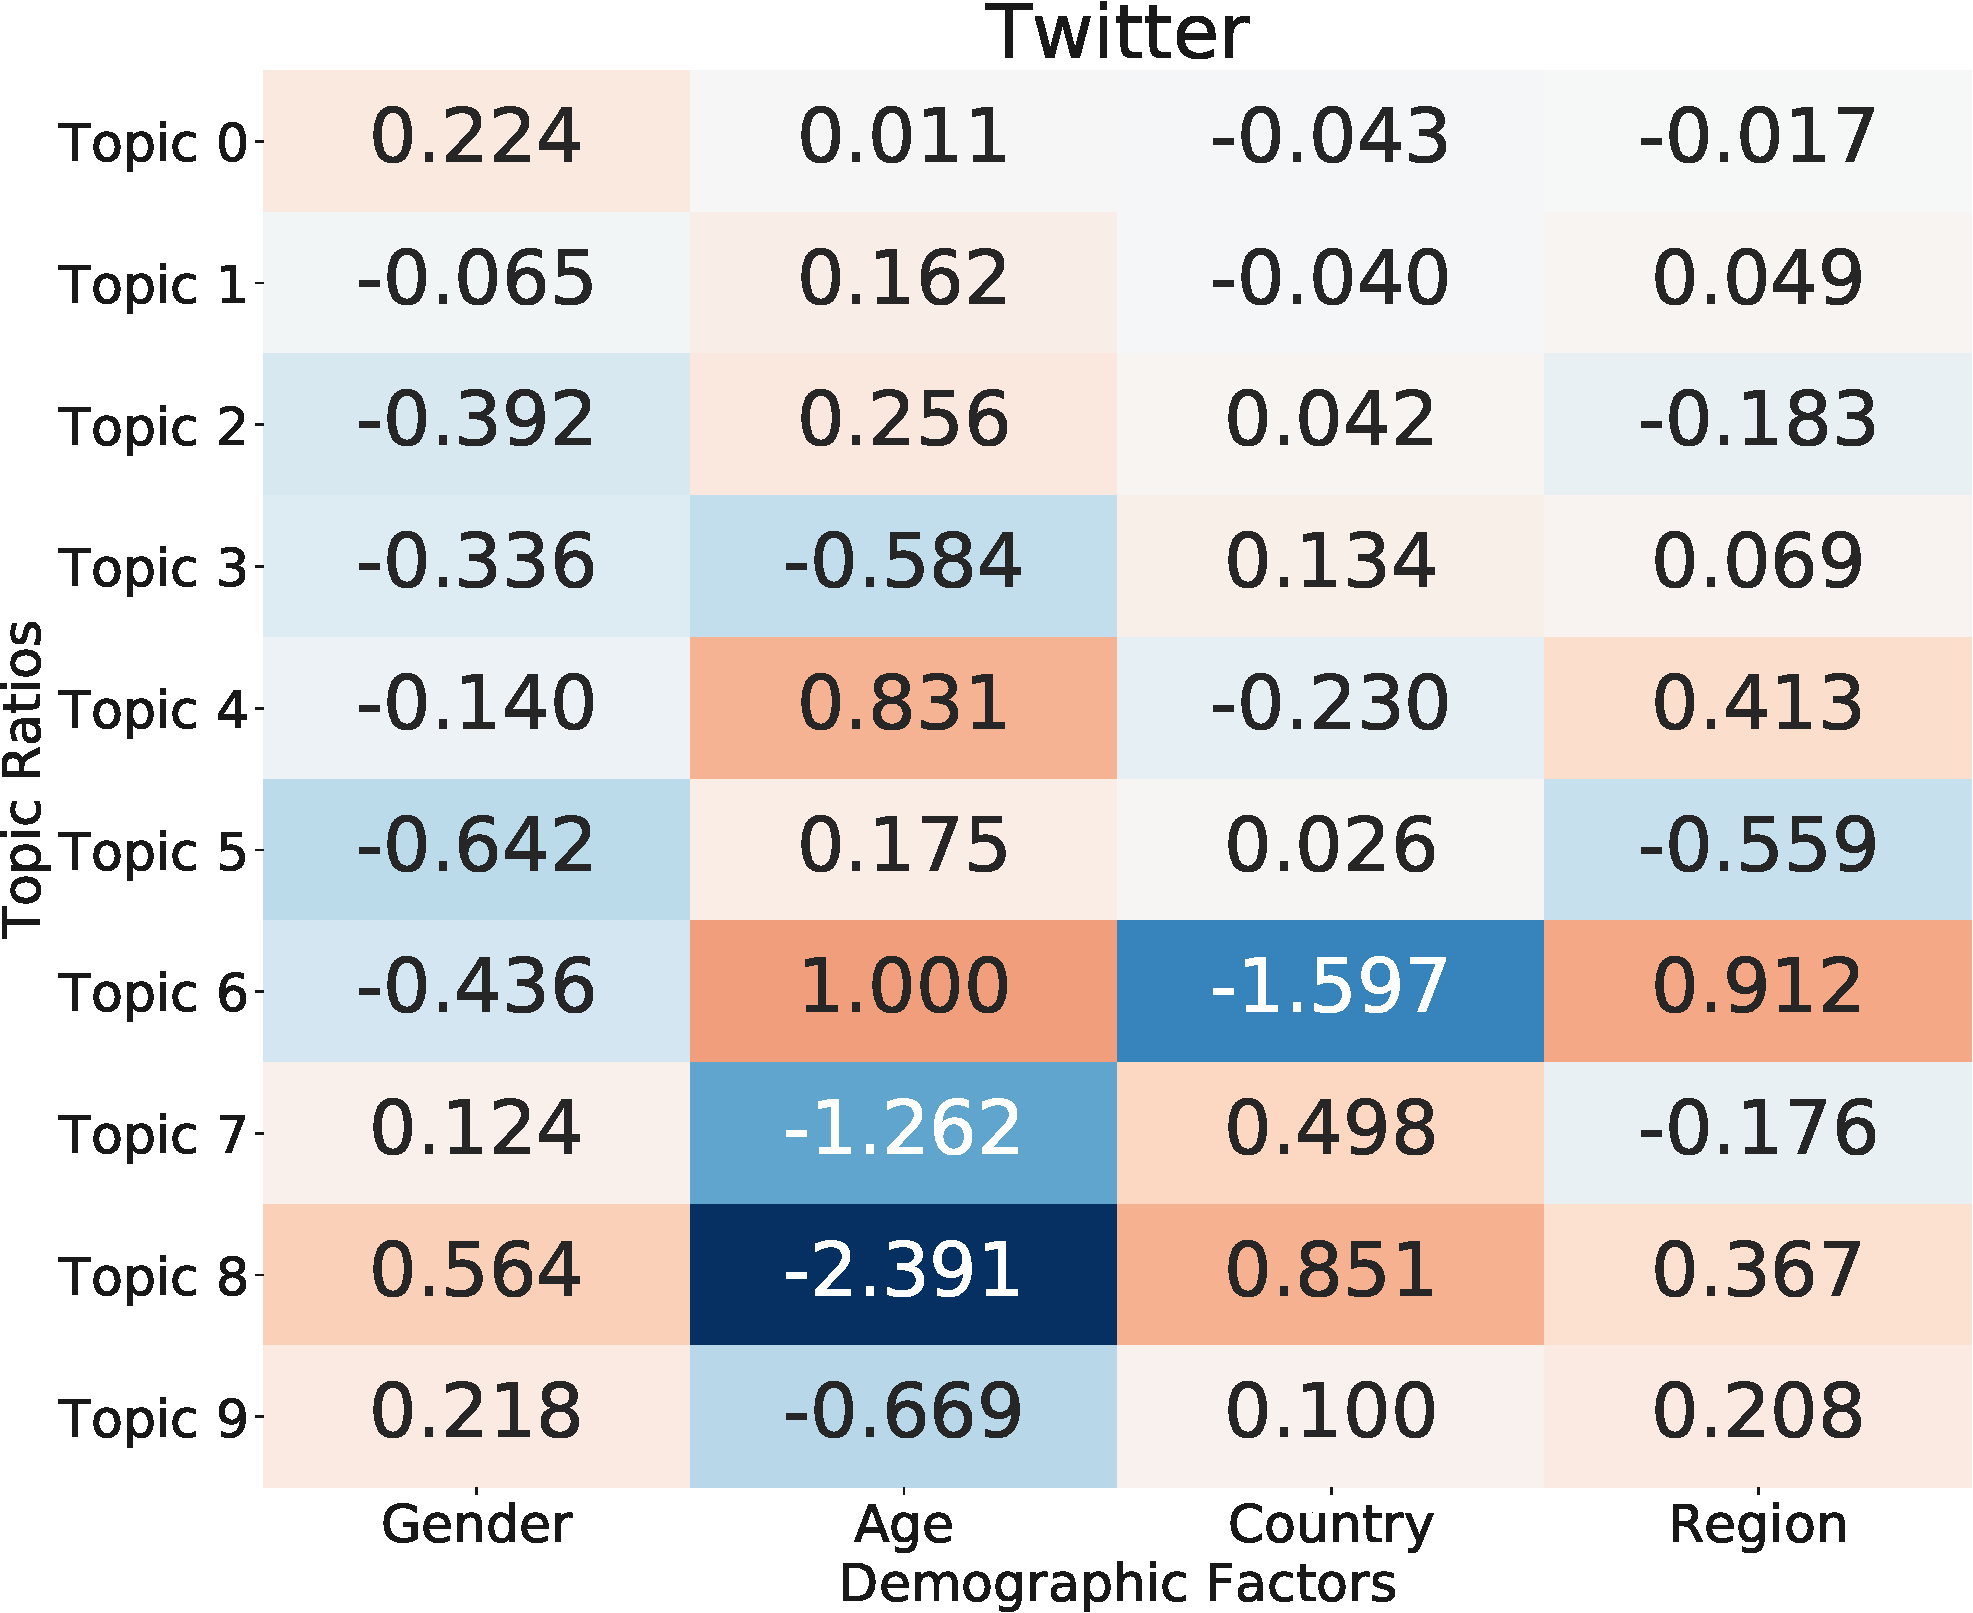
\includegraphics[width=0.44\textwidth]{./images/chapter4/twitter_ratio.pdf}
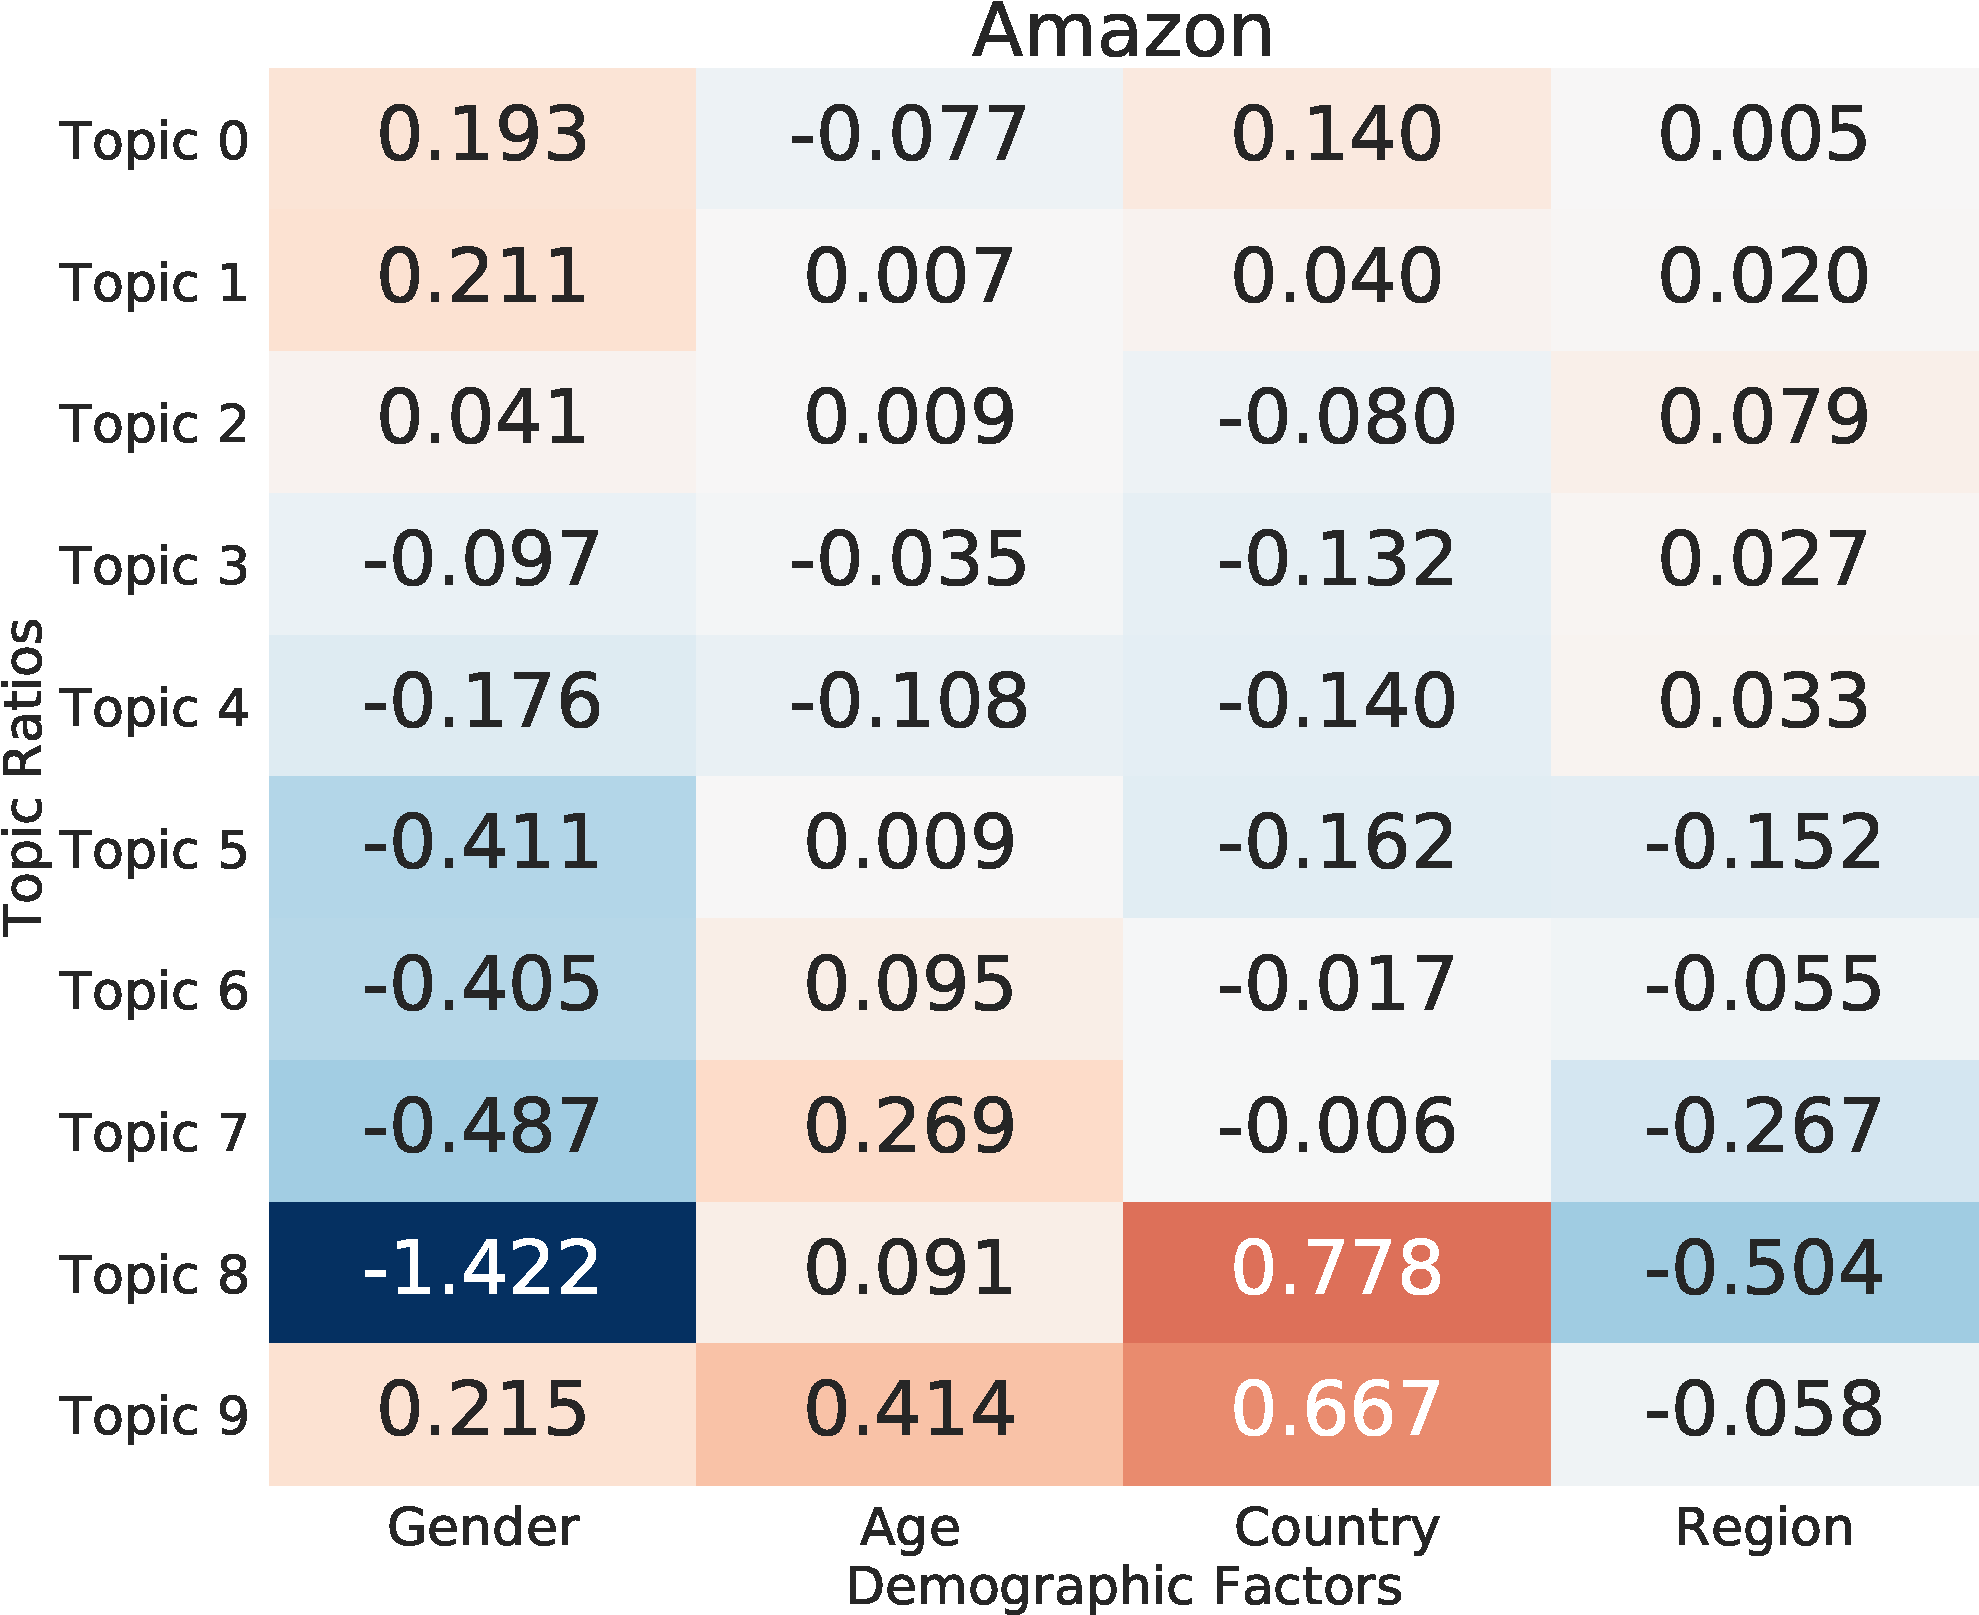
\includegraphics[width=0.44\textwidth]{./images/chapter4/amazon_ratio.pdf}
\newline
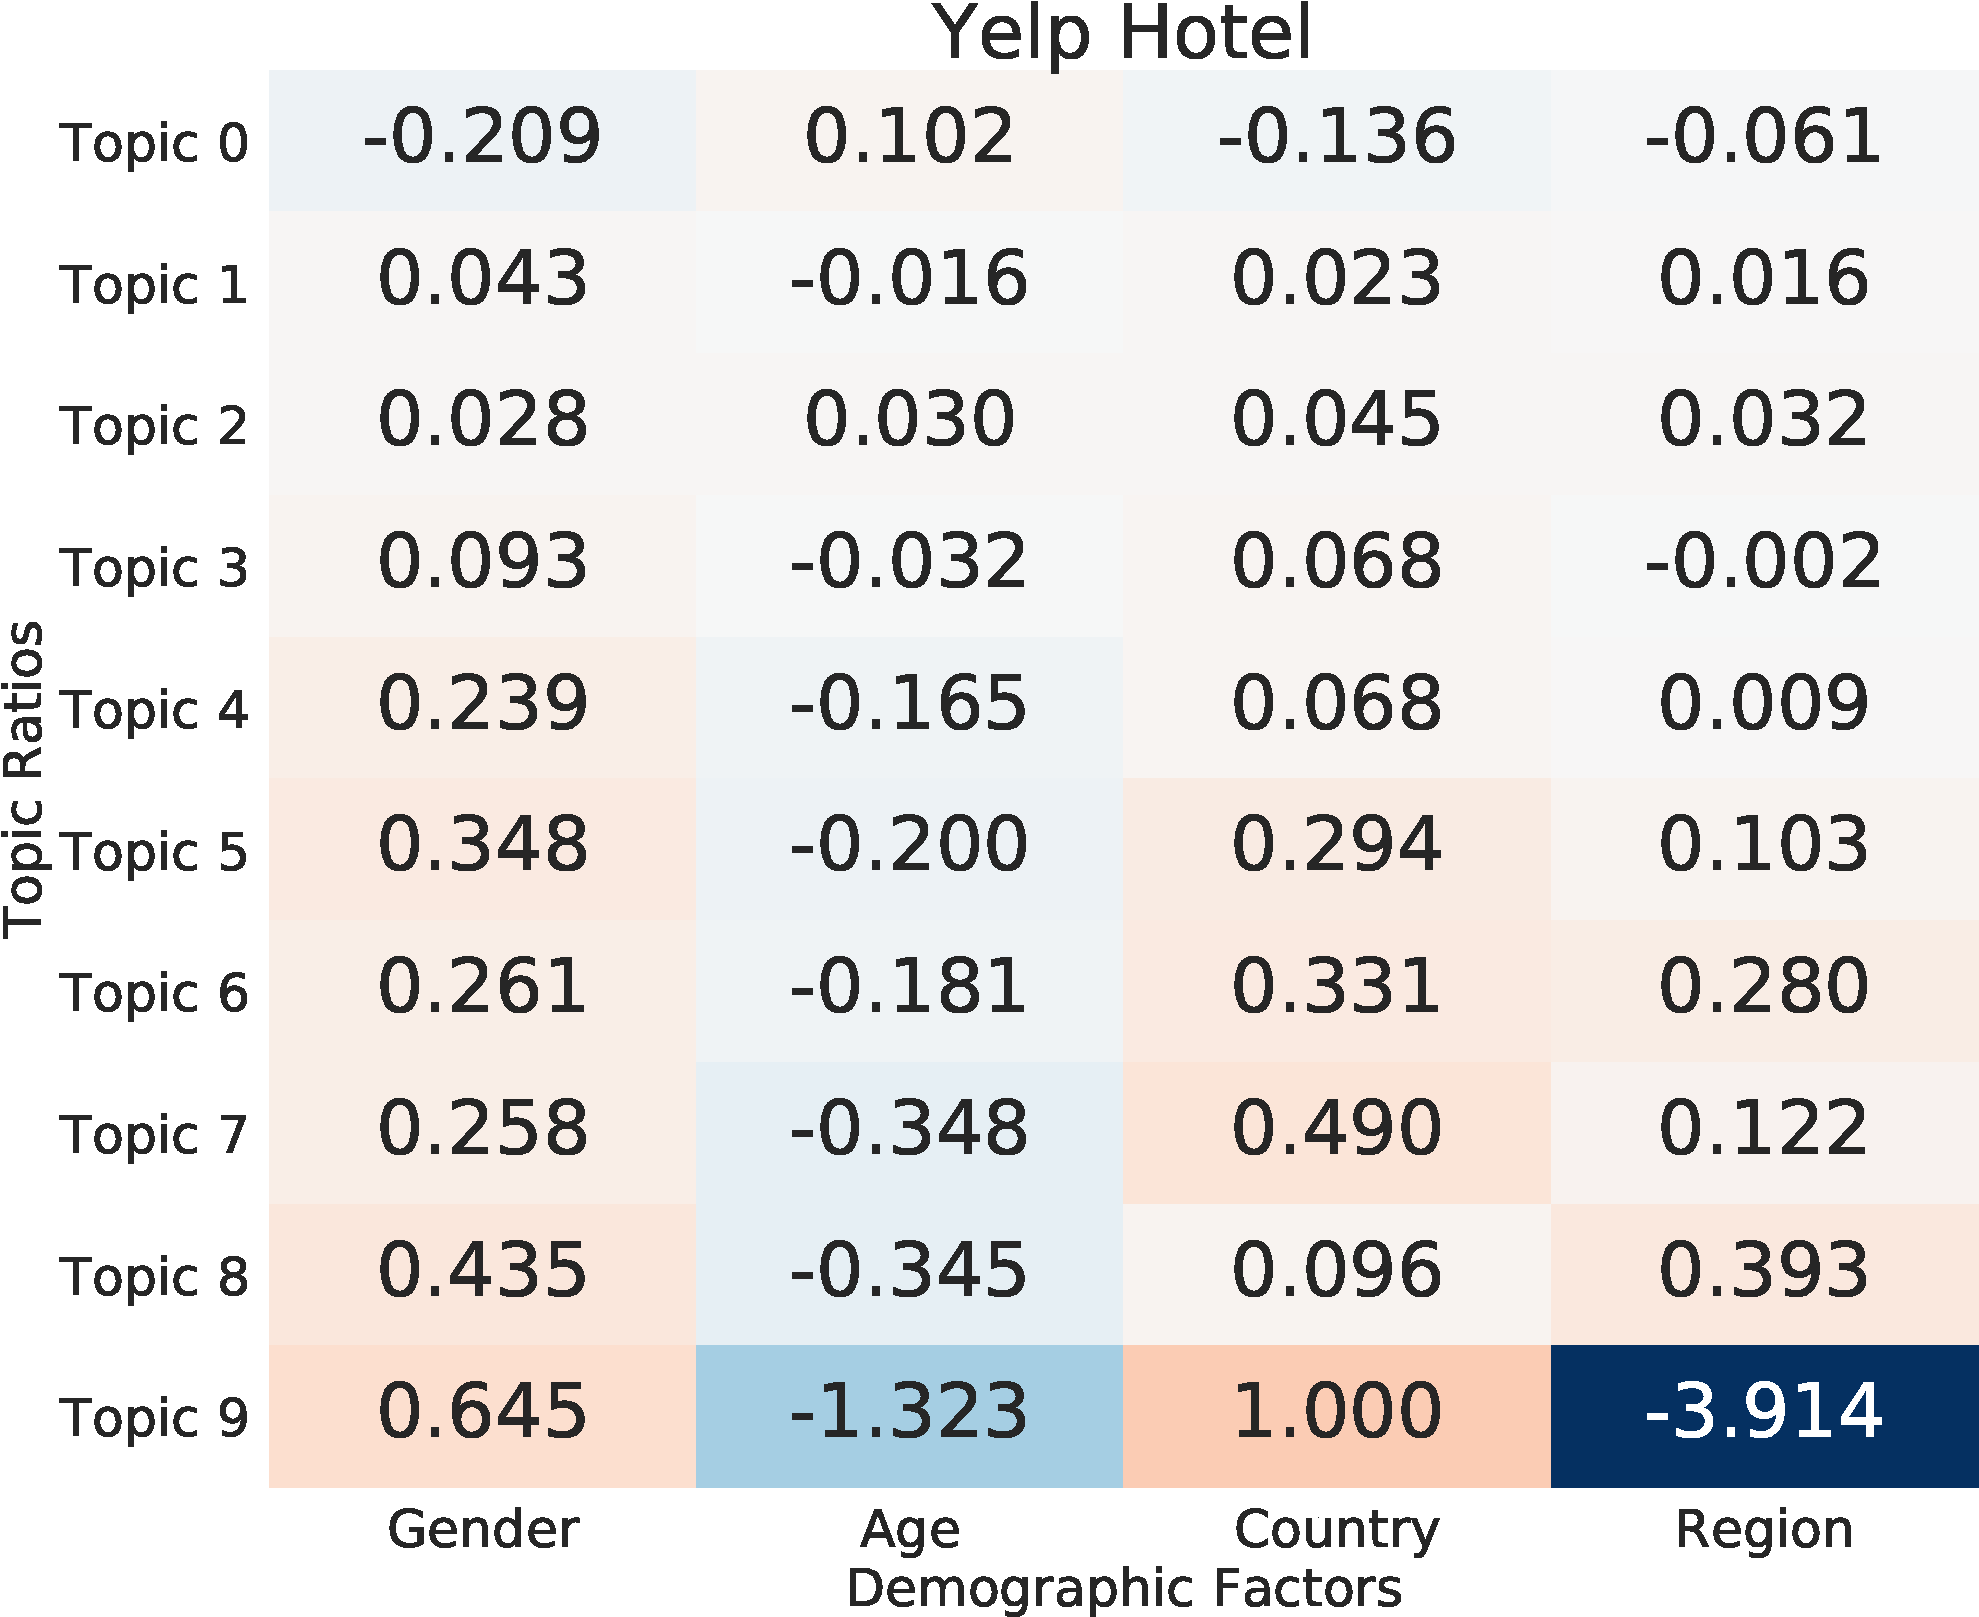
\includegraphics[width=0.44\textwidth]{./images/chapter4/yelp_hotel_ratio.pdf}
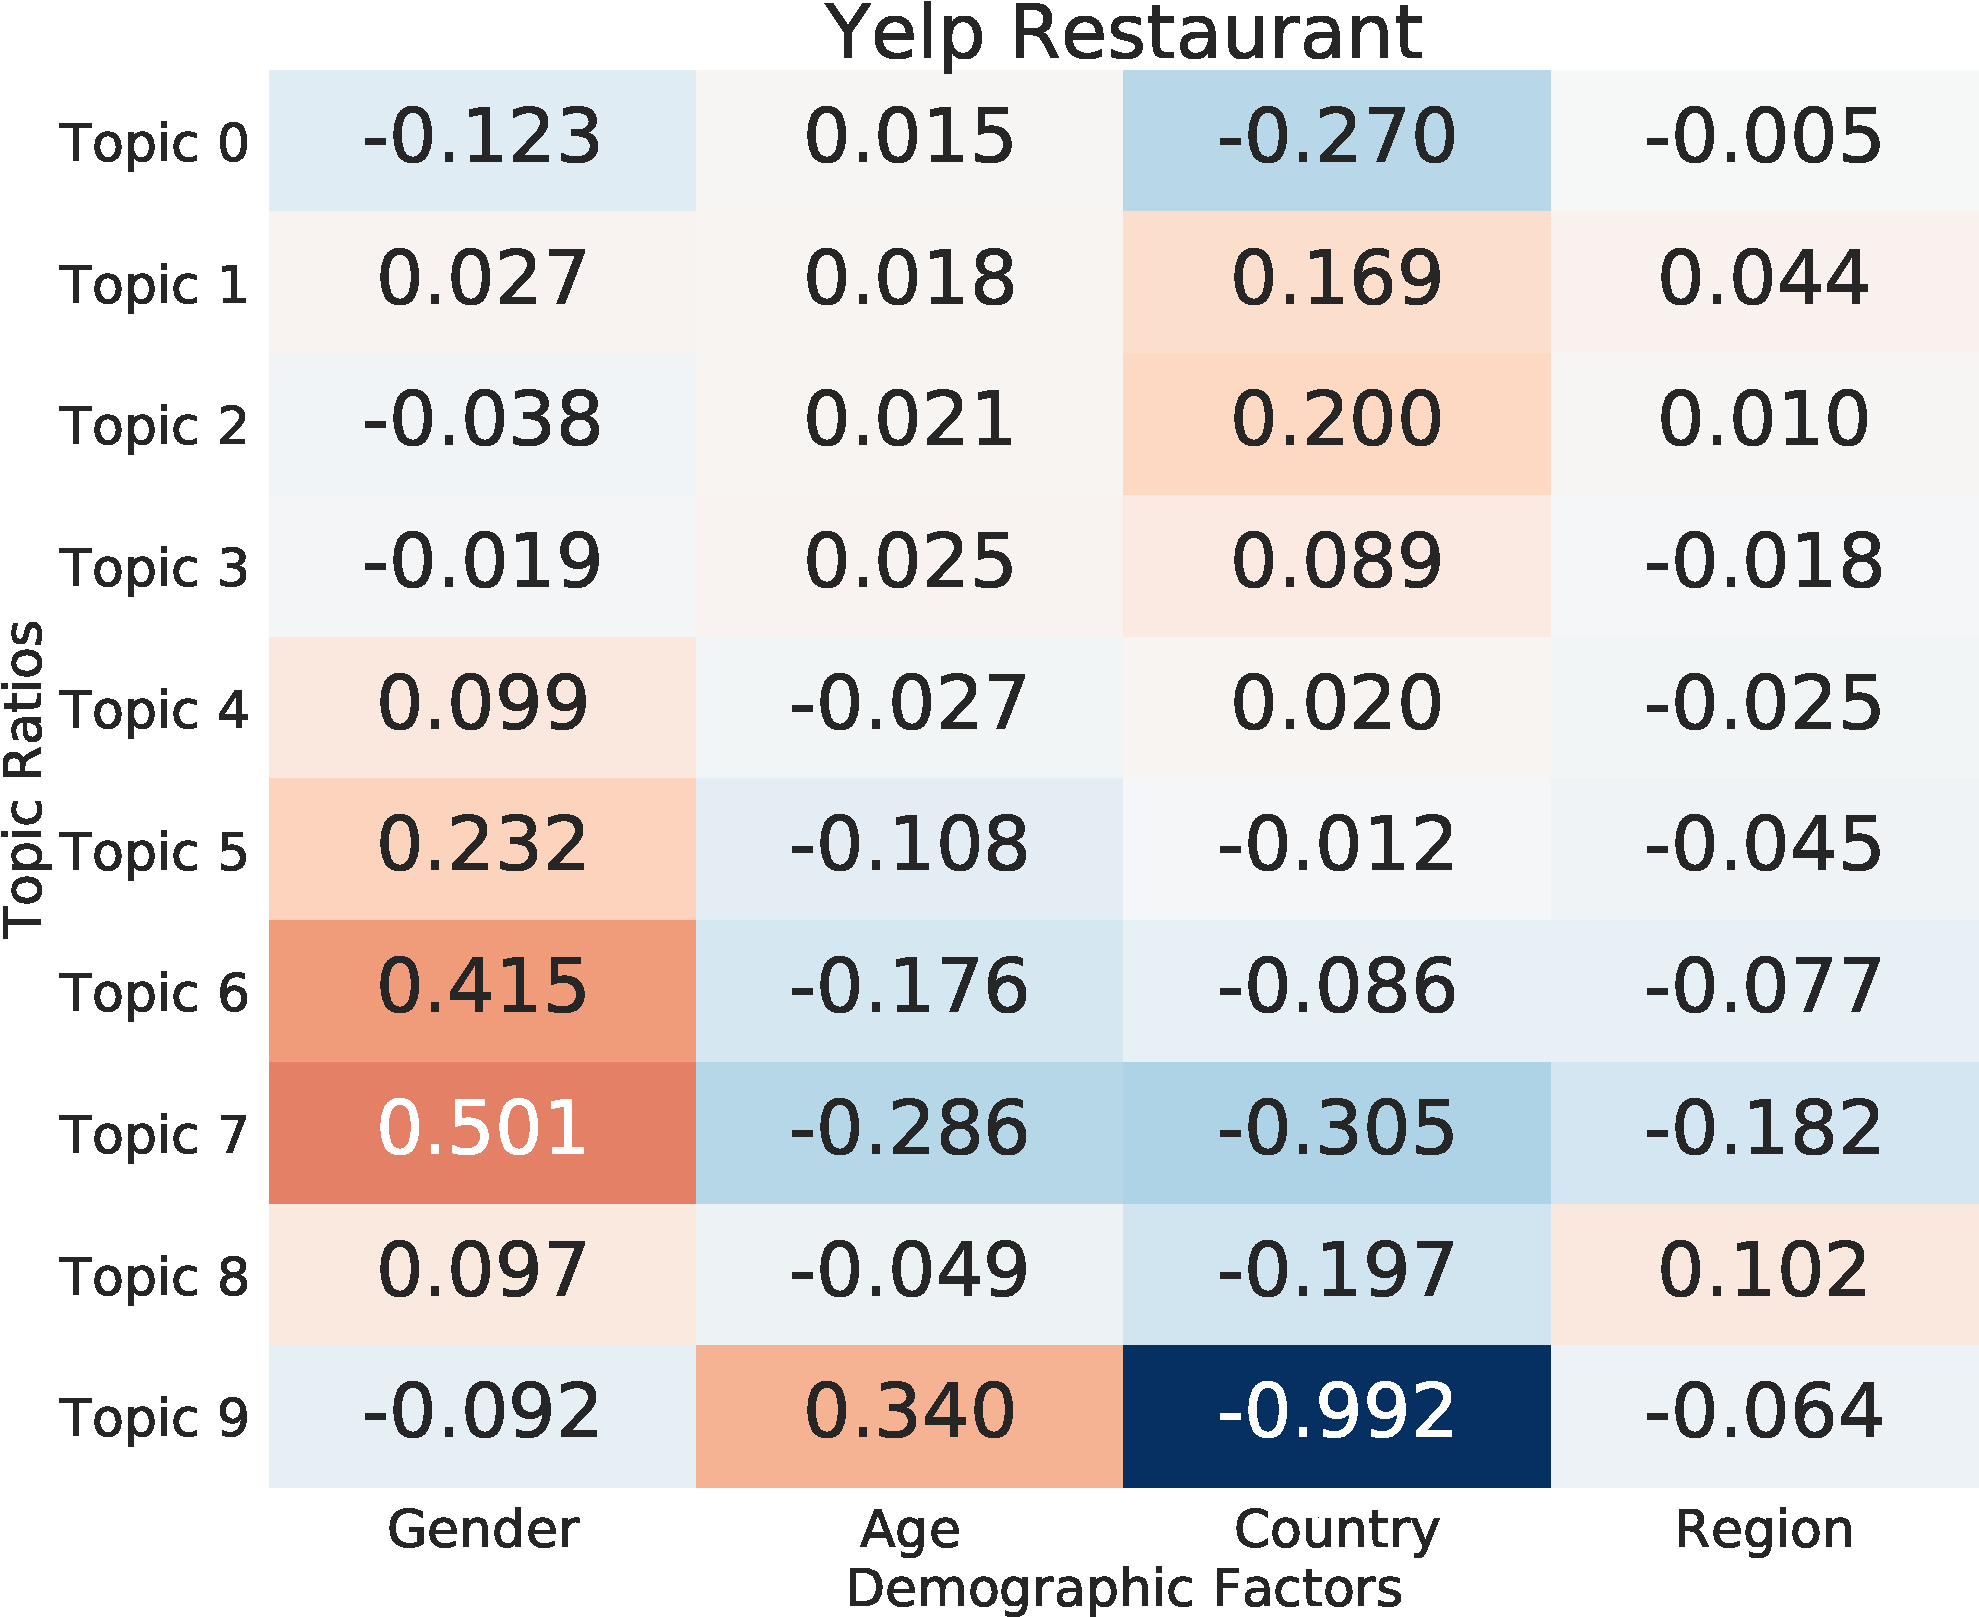
\includegraphics[width=0.44\textwidth]{./images/chapter4/yelp_rest_ratio.pdf}
\caption{Topic distribution log ratios. % for the Twitter, Amazon, Yelp Hotel and Yelp Restaurant data (from left to right) 
A value of 0 means that demographic groups use that topic in equal amounts, while values away from 0 mean that the topic is discussed more by one demographic group than the other group(s) in that factor.
}
\label{fig:vary}
\end{figure*}

We additionally examine how the distribution of text content varies across demographic groups. To characterize the content, we represent the text with a topic model.
We trained a Latent Dirichlet Allocation~\cite{blei2003latent} model with 10 topics using GenSim~\cite{rehurek2010software} with default parameters.
After training the topic model, each document $d$ is associated with a probability distribution over the 10 topics. 
The model learns a multinomial topic distribution $P(Z|D)$ from a Dirichlet prior, where $Z$ refers to each topic and $D$ refers to each document.
For each demographic group, we calculate the average topic distribution across the documents from that group.
Then within each factor, we calculate the log-ratio of the topic probabilities for each group.
For example, for topic $k$ for the gender factor,
we calculate $\log_2 \frac{P(Topic=k|Gender=\textrm{female})}{P(Topic=k|Gender=\textrm{male})}$.
The sign of the log-ratio indicates which demographic group is more likely to use the topic.
We do this for all factors;
for region, we simply binarize the four values for the purpose of this visualization (MW + W vs. NE + S).
Results are shown in Figure~\ref{fig:vary}.

%The model generates a multinomial topic distribution $P(Z|D)$ from a Dirichlet prior, where $Z$ is the topic distribution, and the D refers to documents. Particularly, we are interested in how the Z varies among gender ($P(Z|D, G)$), age ($P(Z|D, A)$), country ($P(Z|D, C)$) and region ($P(Z|D, R)$). We associated each document with one topic (the most likely topic in the document) and then calculated the proportion of each topic as the proportion of documents assigned to that topic. Next, to compare linguistic patterns, we calculate the ratios of each topic between types of the demographic factors: gender (female vs. male), age (young vs. old), country (US vs. no-US) and region (MW + W vs. NE + S). For example, we obtain male vs. female by $\frac{P(Z|D, female)}{P(Z|D, male)}$. Finally, we can visualize the extent to which the ratios of 10 topics varies by the four demographic attributes. We show the details in the Figure~\ref{fig:vary}.

The topic model was trained without removing stop words, in case stop word usage varies by group.
However, because of this, the topics all look very similar and are hard to interpret, so we do not show the topics themselves.
What we instead want to show is the degree to which the prevalence of some topics varies across demographic attributes, which are extracted independently from the text used to train the topic models.
We see that while most topics are fairly consistent across demographic groups, most datasets have at least a few topics with large differences.

%\cite{hovy2015demographic} show that demographic variations could associate with their linguistic behaviors online. To understand how linguistic behavior varies among the different demographic groups, we qualitatively examined and characterized how the distribution of content changes across the demographic attributes. 




%MP: Much of this text I included earlier, so now I am commenting it all out...


%\textbf{By gender} (G), $P(Z|D, G)$. Language styles highly associated with the gender of online users~\cite{hovy2018capturing}. The Figure~\ref{fig:vary} shows there are obvious variations between male (left stacked bar) and female (right stacked bar). The Twitter topic distributions are more on the first topic. We infer the reason might be the data is highly focused on ``flu vaccine''.
%

%\textbf{By age} (A), $P(Z|D, A)$. Some people change their linguistic styles as they age~\cite{wagner2012age}. We could partially confirm such a claim in our collected Twitter, Amazon and Yelp hotel data, which show more fluctuations of topic distributions. However, there are fewer variances in the Yelp restaurant data. 
%

%\textbf{By country} (C), $P(Z|D, C)$. From the third column of Figure~\ref{fig:vary}, we could observe that there are more significant variations in the Yelp restaurant data than other sources. It might be that people from different countries might express opinions in different ways. 
%

%\textbf{By region} (R), $P(Z|D, R)$. Goel et al.~\cite{goel2016social} show in online social media there are significantly different linguistic styles across different US regions. For example, due to English dialects among US regions, people in the Southern US use ``dese'' as ``these'' and people in Baltimore use ``ard'' as ``alright''. We might observe almost no variations in the Twitter data, which might be that people usually report ``flu vaccine'' in a similarly formal way. In contrast, we could observe that people talk more differently in the Amazon music data. 
%

\subsection{Are Document Categories Expressed Differently by Different User Groups?}

While text content varies across different user groups,
it is a separate question whether those variations will affect document classification.
For example, if men and women discuss different topics online,
but express sentiment in the same way,
then those differences will not affect a sentiment classifier.
Prior work has shown that the way 
people express opinions in online social media 
does vary by gender, age, geographic location, and political orientation~\cite{hinds2018demographic};
thus, there is reason to believe that concepts like sentiment will be expressed differently by different groups.
As a final exploratory experiment,
we now consider whether the text features that are predictive of
document categories (e.g., positive or negative sentiment)
also vary with user factors.

\begin{figure}[tb!]
\centering
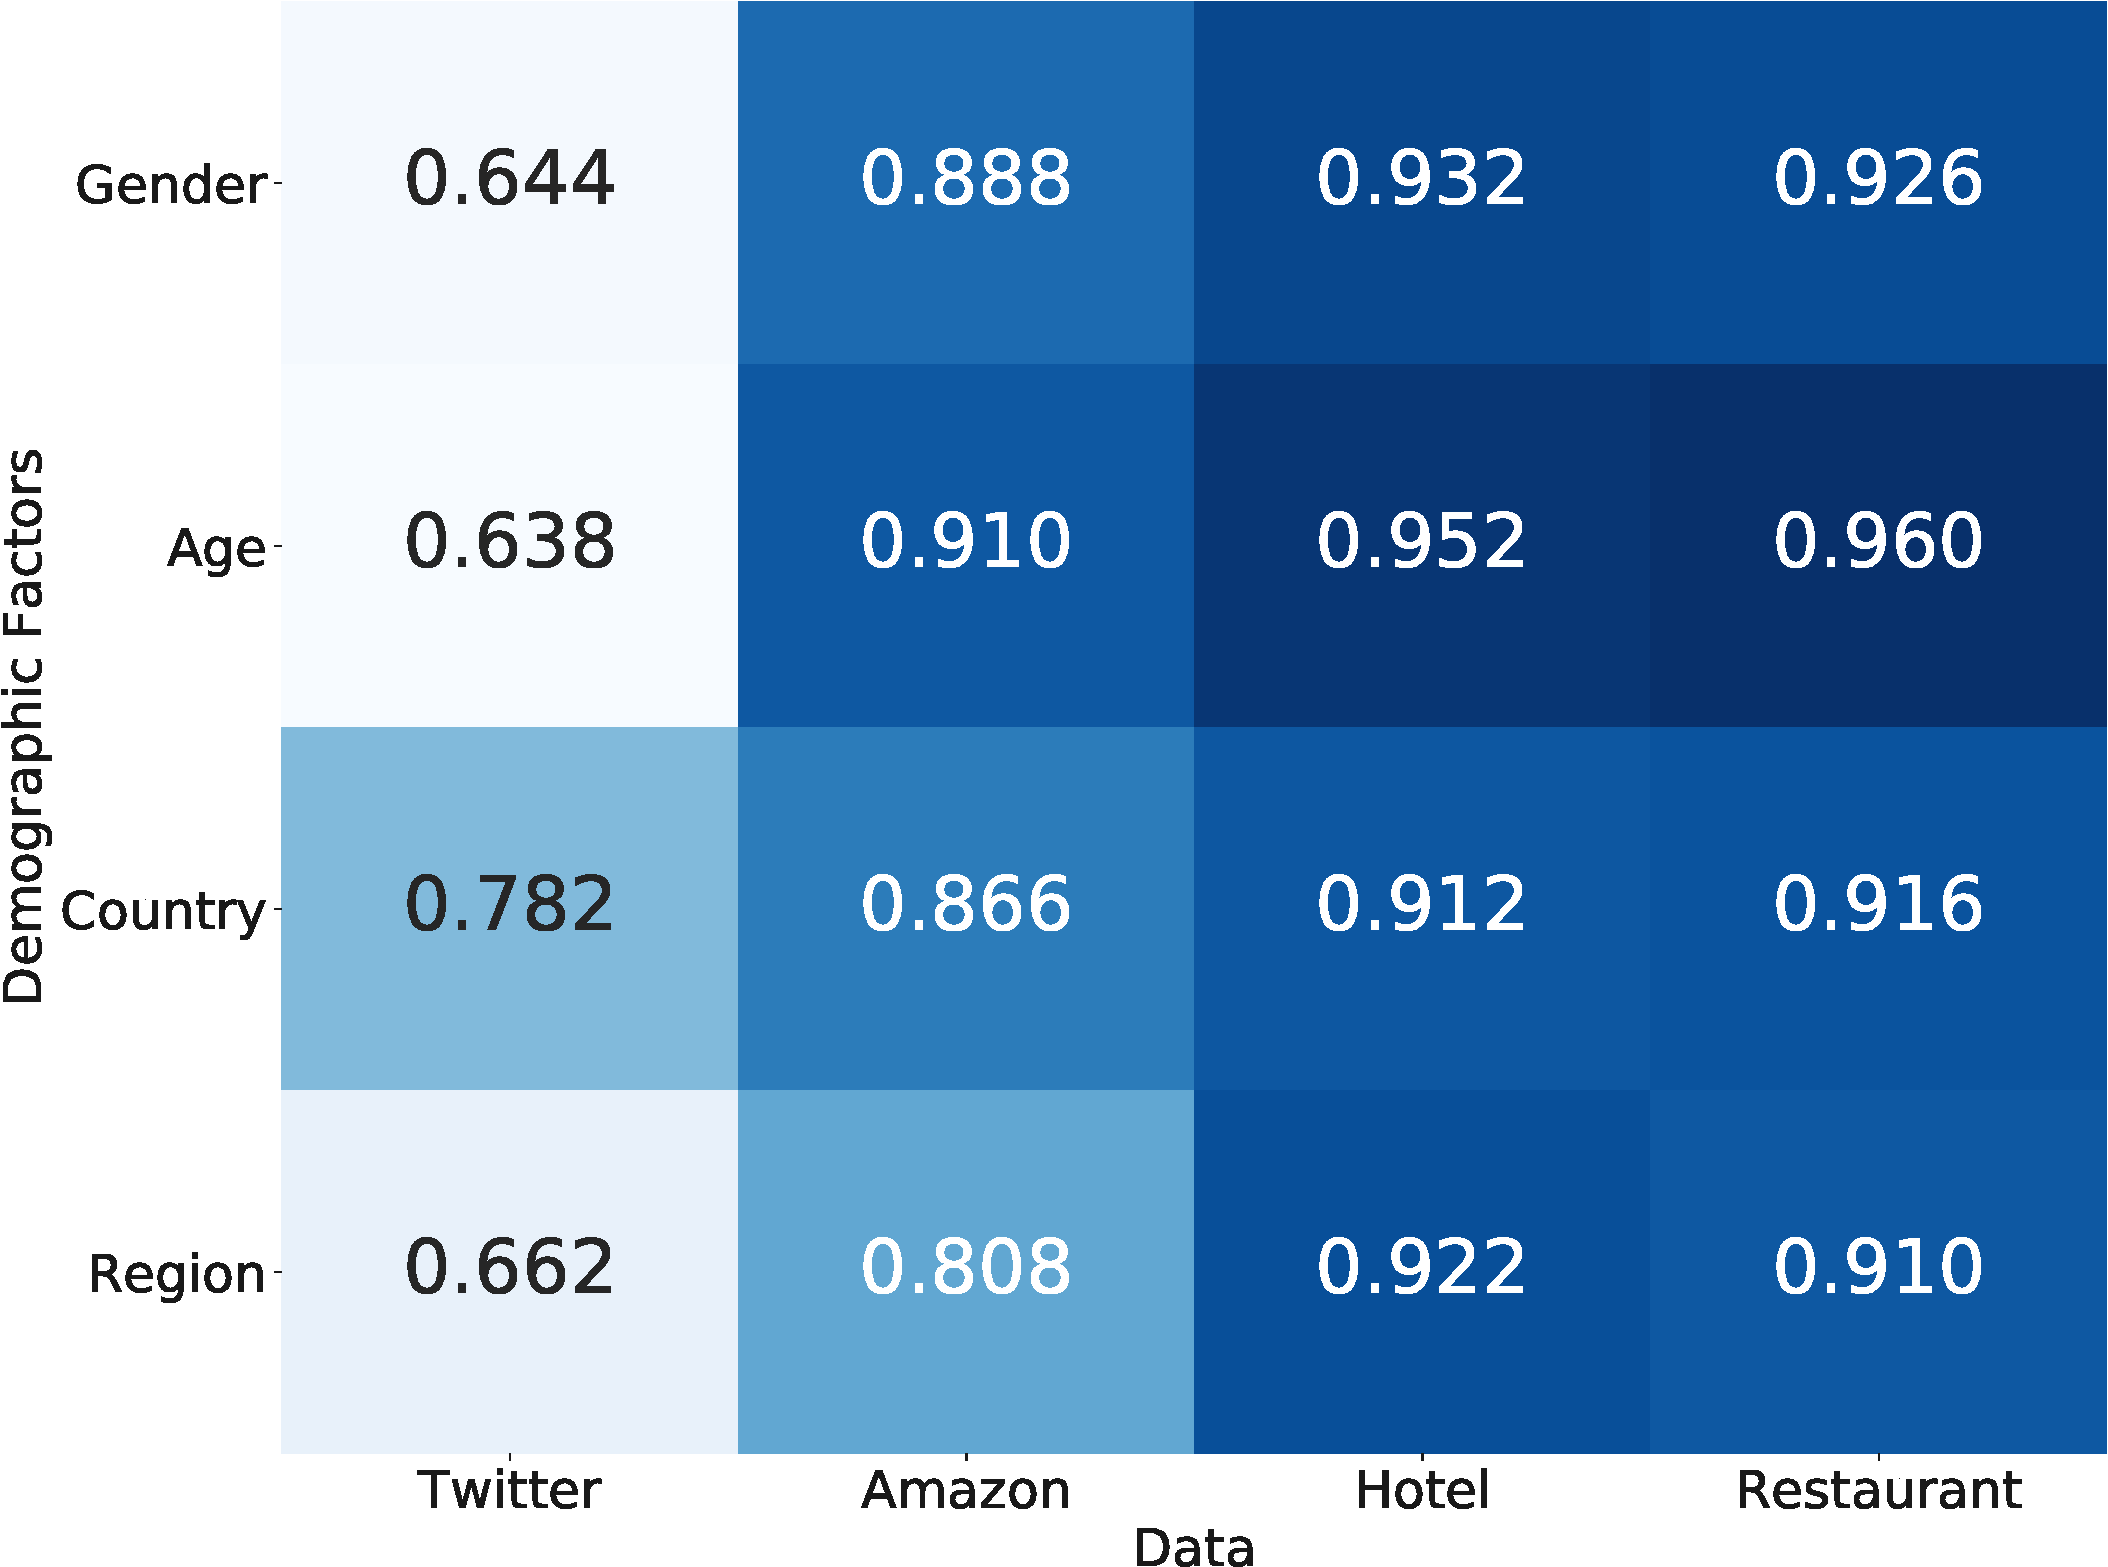
\includegraphics[scale=0.30]{./images/chapter4/overlap.pdf}
\caption{Overlap in most predictive classification features across different demographic groups, calculated for each demographic factor and each dataset. Darker color indicates less variation in word usage across demographic groups.
}
\label{fig:overlap}
\end{figure}

To compare how word expressions vary among the demographic factors, we conduct a word-level feature comparison.
For each demographic group, we collect only documents that belong to that group and then calculate the n-gram features (same features as in Section~\ref{subsec:analysis}) that are most associated with the document class labels.
Using mutual information, we select the top 1,000 features for each attribute.
Then within each demographic factor (e.g., gender),
we calculate the percentage of top 1,000 features that overlap across the different attribute values in that factor (e.g., male and female).
Specifically, if $S_0$ is the set of top features for one attribute and $S_1$ is the set of top features for another attribute, the percent overlap is calculated as $|S_0 \cap S_1|/1000$.
Results are shown in Figure~\ref{fig:overlap}. 
Lower percentages indicate higher variation in how different groups express the concepts being classified (e.g., sentiment).
The Twitter data shows the most variation while the Yelp hotel data shows the least variation.



\begin{figure*}[htp]
\centering
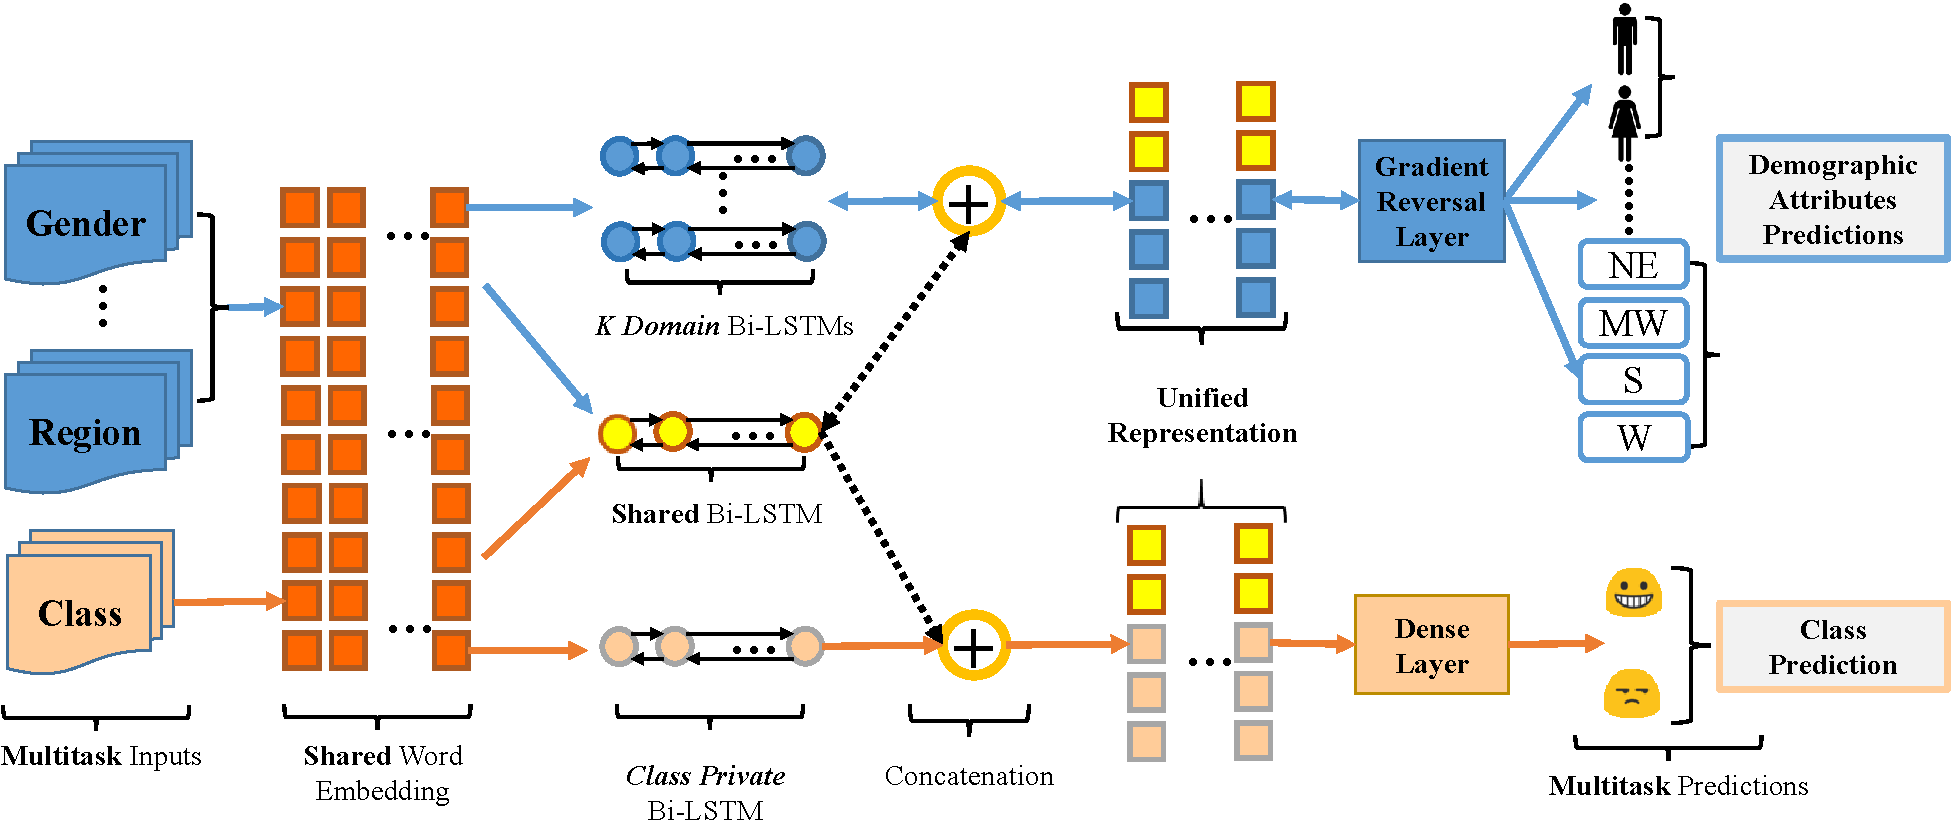
\includegraphics[scale=0.47]{./images/chapter4/model.pdf}
\caption{Neural User Factor Adaptation (NUFA) model. 
%``Class'' refers to the class labels of the documents, which are binary-valued. 
NUFA optimizes for two major tasks, demographic prediction (blue blocks and arrows) and text classification (light orange blocks and arrows). 
During the training phase, documents labeled with demographic information go through the demographic classifier, and documents with class labels go through the document classifier. 
This helps NUFA learn representations that are useful for classifying documents versus representations that are useful for predicting demographics.
At test time, documents are given only to the document classifier, leaving out the demographic classifiers. 
%In this way, NUFA could adapt user demographic knowledge into the text classifier.
}
\label{fig:model}
\end{figure*}

\subsection{Model}
\label{sec:model}

Models for user factor adaptation generally treat
this as a problem of {\em domain adaptation}~\cite{volkova2013exploring,lynn2017human}.
Domain adaptation methods are used to learn models that can be applied to data whose distributions may differ from the training data.
Commonly used methods include feature augmentation~\cite{daume2007frustratingly, joshi2013s, huang2018examining}
and structural correspondence learning~\cite{blitzer2006domain},
while recent approaches rely on 
domain adversarial training~\cite{ganin2016domain, chen2016adversarial, liu2017adversarial, huang2018modeling}. 
We borrow concepts of domain adaptation to construct a model that is robust to variations across user factors.


In our proposed {\bf Neural User Factor Adaptation (NUFA)} model, we treat each variable of interest (demographic attributes and document class label) as a separate, but jointly modeled, prediction task.
%additionally, we treat each demographic attribute as a domain for the purpose of adaptation. 
The goal is to perform well at predicting document classes, while the demographic attribute tasks are modeled primarily for the purpose of learning characteristics of the demographic groups.
%Our primary goal is to learn to account for user demographic information in a way that improves the performance of the document classification model. 
Thus, the model aims to learn discriminative features for text classification while learning to be invariant to the linguistic characteristics of the demographic groups. 
Once trained, this classifier can be applied to test documents without requiring the demographic attributes.

Concretely, we propose the multitask learning framework in Figure~\ref{fig:model}. 
The model extracts features from the text for the demographic attribute prediction tasks and the classification task, as well as joint features for all tasks in which features for both demographics and document classes are mapped into the same vector space.
%\textcolor{red}{We employ a shared embedding feature extractor to map both features from demographic attributes and document classes into the same vector space, which aims to keep the model from being distracted by different input sources.}
Each feature space is constructed with a separate Bidirectional Long Short-Term Memory model (Bi-LSTM)~\cite{hochreiter1997long}.

Because language styles vary across groups, as shown in Section~\ref{subsec:analysis}, information from each task could be useful to the other.
Thus, our intuition is that while we model the document and demographic predictions as independent tasks, the shared feature space allows the model to transfer knowledge from the demographic tasks to the text classification task and vice versa. 

However, we want to keep the feature space such that
the features are predictive of document classes in a way that is invariant to demographic shifts. 
To avoid learning features for the document classifier that are too strongly associated with user factors, 
we use adversarial training.
The result is that the demographic information is encoded primarily in the features used for the demographic classifiers, while learning invariant text features that work {\em across} different demographic groups for the document classifier. 

%\vspace{-1ex}
\paragraph{Domain Sampling and Model Inputs.} 
Our model requires all domains (demographic attributes) to be known during training, but not all attributes are known in our datasets.
Instead of explicitly modeling the missing data,
we simply sample documents where all user attributes of interest are available.
At test time, this limitation does not apply because only the document text is required as input to the document classifier.

%We feed the inputs with all text documents. However, one issue with user demographic label in the real world is ``missing labels'', for example, a user might not provide any private information. Moreover, we could not do the same training steps that proposed in the previous research~\cite{chen2016adversarial} that treats sampled training data as positive and test data as negative. Because they do not have ``missing labels'' issue and in our scenario, demographic labels are well uniformly distributed in both training and test data. Therefore, we sample a batch of documents that have labels for each demographic prediction task. Noted that we only feed data to the document classifier during the test stage.

%\vspace{-1ex}
\paragraph{Shared Embedding Space.} We use a common embedding layer for both document and demographic factor predictions. The goal is that the trained embeddings will capture the language variations that are associated with the demographic groups as well as document labels. Parameters are initialized with pre-trained  embeddings~\cite{mikolov2013distributed, pennington2014glove}.

%\vspace{-1ex}
\paragraph{K+2 Bi-LSTMs.} We combine ideas from two previous works on domain adaptation~\cite{liu2017adversarial, kim2017domain}. Kim et al.~\cite{kim2017domain} proposed $K$$+$$1$ Bi-LSTMs, where $K$ is the number of domains, and Liu et al.~\cite{liu2017adversarial} proposed to combine shared and independent Bi-LSTMs for each prediction task. In our model, we create one independent Bi-LSTM for each demographic domain (blue), one independent Bi-LSTM for the document classifier (orange), and one shared Bi-LSTM that is used in both the demographic prediction and document classification tasks (yellow). The intuition is to transfer learned information to one and the other through this shared Bi-LSTM while leaving some free spaces for both document label and demographic factors predictions. We then concatenate outputs of the shared LSTM with each task-independent LSTM together. This helps the text classifier capture demographic knowledge.

%\vspace{-1ex}
\paragraph{Demographic Classifier.} 
We adjust the degree to which the demographic classifiers can discriminate between attributes. 
To find a balance between the invariant knowledge and differences across user demographic factors, we apply domain adversarial training~\cite{ganin2016domain} (the blue block indicating the ``gradient reversal layer'') to each domain prediction task. The predictions use the final concatenated representations, where the prediction is modeled with a {softmax} function for the region and a binary {sigmoid} function for the other user demographic factors. 

%\vspace{-1ex}
\paragraph{Document Classifier.} We feed the concatenated outputs of the document and shared Bi-LSTMs to one layer feed-forward network (the orange block indicating the ``dense layer''). Finally, the document classifier outputs a probability via a sigmoid.

%\vspace{-1ex}
\paragraph{Joint Multitask Learning.} We use the categorical cross-entropy loss to optimize the $K+1$ prediction tasks jointly. One question is how to assign importance to the multiple tasks. Because our target is document classification, we assign a cost to the domain prediction loss ($L_{domain}$). Each prediction task has its own weight, $\alpha_k$. The final loss function is defined as $L = L_{doc} + \sum_{k=1}^K \alpha_k L_{domain, k}$. In summary, the proposed model learns and adapts to user demographic factors through three aspects: shared embeddings, shared Bi-LSTMs, and joint optimization.

\subsection{Experiments}
\label{sec:experiments}
  
We experiment with document classification on our four corpora using various models. Our goal is to test whether models that adapt to user factors can outperform models that do not, and to understand which components of models can facilitate user factor adaptation.
  
\subsubsection{Data Processing}

We replaced hyperlinks, usernames, and hashtags with generic symbols. Documents were lowercased and tokenized using NLTK~\cite{bird2004nltk}. 
The corpora were randomly split into training (80\%), development (10\%), and test (10\%) sets. %, summarized in Table~\ref{table:statics}. 
We train the models on the training set and find the optimal hyperparameters on the development set. We randomly shuffle the training data at the beginning of each training epoch. The evaluation metric is weighted F1 score.

%%MP: This table isn't needed, because you can get the same information from the earlier data table in section 2, and the fact that the data split is 80/10/10.
%
%\begin{table}[ht]
%  \centering
%  \resizebox{\columnwidth}{!}{
%    \begin{tabular}{c|ccc|c}
%     \hline\hline
%     Datasets & Train & Dev. & Test & Total\\
%     \hline
%     Twitter & 7,875 & 984 & 985 & 9,844 \\
%     Amazon & 32,335 & 4,042 & 4,042 & 40,419 \\
%     Hotel & 135,164 & 16,896 & 16,896 & 168,956 \\
%     Restaurant & 570,750 & 71,344 & 71,344 & 713,438 \\
%     \hline
%    \end{tabular}
%    }
%    \caption{Data statistics.}
%    \label{table:statics}
%\end{table}
%
%%

\subsubsection{No Adaptation Baselines}
We compare to three standard classifiers that do not perform adaptation.


%\vspace{-.5ex}
\paragraph{N-gram.} We extract TF-IDF-weighted features of 1-, 2-, and 3-grams on the corpora, using the most frequent 15K features with the minimum feature frequency as 2.
We trained a logistic regression classifier using the \texttt{SGDClassifier} implementation in scikit-learn~\cite{pedregosa2011scikit}
using a batch size of 256 and 1,000 iterations. 

%\vspace{-.5ex}
\paragraph{CNN.} We used Keras~\cite{chollet2015keras} to implement the Convolutional Neural Network (CNN) classifier described in~\cite{kim2014convolutional}. To keep consistent, we initialize the embedding weight with pre-trained word embeddings~\cite{mikolov2013distributed,pennington2014glove}. We only keep the 15K most frequent words and replace the rest with an ``unk'' token. Each document was padded to a length of 50. We keep all parameter settings as described in the paper. We fed 50 documents to the model each batch and trained for 20 epochs.

%\vspace{-.5ex}
\paragraph{Bi-LSTM.} We build a bi-directional Long Short Term Memory (bi-LSTM)~\cite{hochreiter1997long} classifier. The classifier is initialized with the pre-trained word embeddings, and we initialize training with the same parameters used for the NUFA.



\subsubsection{Adaptation Models}

We consider two baseline domain adaptation models that can adapt for user factors, a non-neural method and a neural model.
We then provide the training details of our proposed model, NUFA.
Finally, we consider two variants of NUFA that ablate components of the model, allowing us to evaluate the contribution of each component.

%\vspace{-.5ex}
\paragraph{FEDA.} Lynn et al.~\cite{lynn2017human} used a modification of the ``frustratingly easy'' domain adaptation (FEDA) method~\cite{daume2007frustratingly} to adapt for user factors. 
We use a modification of this method where the four user factors and their values are treated as domains.
We first extract domain-specific and general representations as TF-IDF-weighted n-gram (1-, 2, 3-grams) features. We extract the top 15K features for each domain and the general feature set.
With this method, the feature set is augmented such that each feature has a domain-specific version of the feature for each domain, as well as a general domain-independent version of the feature.
%MP: Cutting these details/examples to save space
%for a total of $1+\sum_{k=1}^{K}C_k$ feature sets, where $C_k$ is the number of categories for the $k$th domain. 
The features values are set to the original feature values for the domain-independent features and the domain-specific features that apply to the document, while domain-specific features for documents that do not belong to that domain are set to $0$.
For example, using gender as a domain, a training document with a female author would be encoded as $[F_{general}, F_{domain, female}, 0]$, while a document with a male author would be encoded as $[F_{general}, 0, F_{domain, male}]$.
Different from prior work with FEDA for user-factor adaptation, 
at test time we only use the general, domain-independent features;
the idea is to learn a generalized feature set that is domain invariant.
This is the same approach we used in recent work using FEDA to adapt classifiers to temporal variations~\cite{huang2018examining}.



%\vspace{-.5ex}
\paragraph{DANN.} We consider the domain adversarial training network~\cite{ganin2016domain} (DANN) on the user factor adaptation task. We use Keras to implement the same network and deploy the same pre-trained word embeddings as in NUFA. We then set the domain prediction as the demographic factors prediction and keep the document label prediction as the default. We train the model with 20 epochs with a batch size of 64. Finally, we use the model at the epoch when the model achieves the best result on the development set for the final model.


%\vspace{-0.5ex}
\paragraph{NUFA.}
We initialize the embedding weights by the pre-trained word embeddings~\cite{mikolov2013distributed, pennington2014glove} with 200 dimensional vectors. All LSTMs are fixed outputs as 200-dimension vectors. We set the dropout of LSTM training to 0.2 and the flip gradient value to .01 during the adversarial training. The dense layer has 128 neurons with ReLU activation function and dropout of 0.2. User factors and document label predictions are optimized jointly using Adam~\cite{kingma2014adam} with a learning rate of 0.001 and batch size of 64. We train NUFA for up to 20 epochs and select the best model on the development set. 
For single-factor adaptation (next section), we set $\alpha$ to 0.1;
for multi-factor adaptation, we use a heuristic for setting $\alpha$ described in that section.
We implemented NUFA in Keras~\cite{chollet2015keras}.

%\vspace{-0.5ex}
\paragraph{NUFA--s.} To understand the role of the shared Bi-LSTM in our model, we conduct experiments on NUFA without the shared Bi-LSTM. We follow the same experimental steps as NUFA and denote it as NUFA$-$s (NUFA minus shared Bi-LSTM). %\textcolor{red}{This will enforce separated training process of the prediction tasks and directly impacts the shared embedding layer.}

%\vspace{-0.5ex}
\paragraph{NUFA--a.} To understand the role of the adversarial training in our model, we conduct experiments of the NUFA without adversarial training, denoted as NUFA$-$a (NUFA minus adversarial).



\begin{table}[tb!]
\centering
\begin{tabular}{c|c|c|c|c}
 & Twitter & Amazon & Hotel & Rest. \\\hline
 \multicolumn{5}{c}{No Adaptation} \\\hline
N-gram & .866 & .793 & .857 & .866 \\
CNN & .879 & .776 & .825 & .846 \\
Bi-LSTM & .869 & .776 & .842 & .875 \\\hline
\multicolumn{5}{c}{Adaptation (Gender)} \\\hline
FEDA & .814 & .809 & \textbf{.865} & .874 \\
DANN & .864 & .832 & .813 & .855 \\ \hline
NUFA$-$s & .880 & \em .845 & .857 & .869 \\
NUFA$-$a & .874 & .842 & .852 & .868 \\
NUFA & \em .886 & .844 & .854 & \textbf{.881} \\ \hline
\multicolumn{5}{c}{Adaptation (Age)} \\\hline
FEDA & .813 & .801 & \bf .865 & .873 \\
DANN & .856 & .824 & .811 & .851 \\ \hline
NUFA$-$s & .872 & \em .843 & .850 & .879 \\
NUFA$-$a & .882 & .841 & .852 & .878 \\
NUFA & \em .885 & .839 & .857 & \em .880 \\ \hline
\multicolumn{5}{c}{Adaptation (Country)} \\\hline
FEDA & .826 & .768 & \bf .865 & .877 \\
DANN & .868 & .828 & .827 & .855 \\ \hline
NUFA$-$s & .882 & \em .844 & .854 & \em .879 \\
NUFA$-$a & .880 & .838 & .855 & .877 \\
NUFA & \textbf{.896} & .843 & .854 & \em .879 \\ \hline
\multicolumn{5}{c}{Adaptation (Region)} \\\hline
FEDA & .826 & .780 & \em .864 & .869 \\
DANN & .875 & .825 & .823 & .852 \\\hline
NUFA$-$s & .874 & .833 & .854 & .878 \\
NUFA$-$a & .882 & .838 & .854 & .875 \\
NUFA & \em .893 & \textbf{.848} & .853 & \em .880\\ \hline
\end{tabular}
\caption{Performance (weighted F1) of no adaptation and single user factor adaptation.
For each dataset, the best score within each demographic domain is italicized; the best score overall is bolded.
}
\label{table:single}
\end{table}

\subsubsection{Results}

\paragraph{Single-Factor Adaptation.} We first consider user factor adaptation for each of the four factors individually. 
Table~\ref{table:single} shows the results.
Adaptation methods almost always outperform the non-adaptation baselines;
the best adaptation model outperforms the best non-adaptation model by $1.5$ to $5.5$ points. 
The improvements indicate that adopting the demographic factors might be beneficial for the classifiers. User factor adaptation thus appears to be important for text classification. 

Comparing the adaptation methods,
our proposed model (NUFA) is best on three of four datasets.
%The Table~\ref{table:single} also shows that our proposed mode with the best result usually outperforms other baselines and particularly exceeds the neural model baseline (DANN) on all datasets. The results show our neural learning framework could effectively learn and adapt the demographic differences into the text classification task. 
On the Hotel dataset, the n-gram model FEDA is always best;
this seems to be a dataset where neural methods perform poorly, since even the n-gram baseline with no adaptation often outperformed the various neural models. 
Whether a neural model is the best choice depends on the dataset,
but among the neural models, NUFA always outperforms DANN.
Finally, the full NUFA model most often outperforms the variants without the shared Bi-LSTM (NUFA$-$s) and without adversarial training (NUFA$-$a). 


\paragraph{Multi-Factor Adaptation.} We experiment with adapting to all four user factors together.
Recall that each domain prediction task in NUFA is weighted by $\alpha_k$.
Initially, we simply used a uniform weighting, $\alpha_k = \alpha/K$,
but we find that we can improve performance with non-uniform weighting.
Because optimizing the $\alpha$ vector would be expensive, 
we instead propose a heuristic that weighs the domains
based on how much each domain is expected to influence the text.
We define $\alpha_k = s_k / (\sum_{k'} s_{k'})$, where $s_k$ is the F1 score of demographic attribute prediction for domain $k$ from Table~\ref{table:explo}.
We denote this method as {\bf NUFA+w}, which refers to this additional weighting process.

\begin{table}[t]
\centering
\begin{tabular}{c|c|c|c|c}
 & Twitter & Amazon & Hotel & Rest. \\\hline
\multicolumn{5}{c}{Baseline Adaptation} \\\hline
FEDA & .806 & .778 & \bf .867 & .869 \\\hline
DANN & .880 & .828 & .830 & .858 \\\hline
\multicolumn{5}{c}{Proposed Model} \\\hline
NUFA & .887 & .848 & .853 & .879 \\
NUFA+w & \bf .901 & \bf .852 & .855 & \bf .885 \\
\end{tabular}
%\vspace{-1ex}
\caption{Results of adaptation for all four user factors.}
\label{table:multi}
\end{table}

Table~\ref{table:multi} shows that combining all user factors
provides a small gain over single-factor adaptation;
the best multi-factor result is higher than the best single-factor result for each dataset.
As with single-factor adaptation, FEDA works best for the Hotel datasets,
while NUFA+w works best for the other three.
Without adding weighting to NUFA, the multi-factor performance is comparable to single-factor performance;
thus, task weighting seems to be critical for good performance when combining multiple factors.



%In this paper, we view the modeling demographic factors as a domain adaptation problem. We integrate the demographic attributes into our text classification model via multitask learning framework.

%MP: I think the background on DA and user factors should probably just be incorporated earlier in the paper when these are first introduced. I can work on doing that when I edit sections 1-2 later.
%XL: I see. I put the related works here because I thought we covered the partially related works in the introduction and the section might not be as important as our proposed method. 

%\textbf{Domain adaptation} tries aligning source with related target distributions to obtain more generalized feature representations and classifiers. For the text classification task, there are two conventional methods, feature augmentations~\cite{daume2007frustratingly, blitzer2006domain, huang2018examining} and domain adversarial training~\cite{ganin2016domain, chen2016adversarial, liu2017adversarial}. However, one issue with the proposed methods is they did not consider the user demographic factors, which show strong variations among social media documents. Additionally, most of the adaptation only work on two different domains, but the demographic factors have more complex domains and divergent differences between domains.

%\textbf{User factor adaptation} integrates demographic factors into the machine learning classifiers. The demographic factors usually refer to the attributes of users, such as gender, age, geographic location, etc. Online generated user texts show demographic variations in the linguistic styles, and the linguistic style differences could be used for the use factor prediction~\cite{rosenthal2011age, zhang2016predicting, hovy2018improving}. The user factors impact on how online users express their opinions and show promising improvements in the text classification task~\cite{volkova2013exploring, hovy2015demographic, lynn2017human, yang2017overcoming}. The closest work to our study~\cite{lynn2017human} created general and domain-specific features to train a more generalized classification model. However, such a method heavily suffers extremely high feature dimensions and handcraft features. 


\section{User Factor Adaptation via User Embedding}

\subsection{Data}

\subsection{Multitask Learning Framework}

\subsection{Experiments}

\subsubsection{User Embedding Evaluation}

\begin{table*}[htp]
\centering
\resizebox{\textwidth}{!}{
    \begin{tabular}{cc||ccc|ccc|ccc}
    \multicolumn{2}{c||}{\multirow{2}{*}{}} & \multicolumn{3}{c|}{Amazon-Health} & \multicolumn{3}{c|}{IMDB} & \multicolumn{3}{c}{Yelp} \\
    \multicolumn{2}{c||}{} & F1@4 & F1@8 & F1@12 & F1@4 & F1@8 & F1@12 & F1@4 & F1@8 & F1@12 \\\hline\hline
    \multirow{5}{*}{Baselines} & word2user &  &  &  &  &  &  &  &  &  \\
     & lda2user &  &  &  &  &  &  &  &  &  \\
     & doc2user &  &  &  &  &  &  &  &  &  \\
     & bert2user &  &  &  &  &  &  &  &  &  \\
     & user2vec &  &  &  &  &  &  &  &  &  \\\hline
    \multirow{3}{*}{Ours} & MTL-global &  &  &  &  &  &  &  &  &  \\
     & MTL-decay &  &  &  &  &  &  &  &  &  \\
     & MTL-local &  &  &  &  &  &  &  &  & 
    \end{tabular}
}
\caption{}
\label{chap4:tab:usereval}
\end{table*}


\subsubsection{Classifier Personalization}


\begin{table*}[htp]
\centering
\begin{tabular}{c||ccc|ccc|ccc}
\multirow{2}{*}{Methods} & \multicolumn{3}{c|}{Amazon-Health} & \multicolumn{3}{c|}{IMDB} & \multicolumn{3}{c}{Yelp} \\
 & Precision & Recall & F1 & Precision & Recall & F1 & Precision & Recall & F1 \\\hline\hline
LR & .834 & .768 & .793 & .818 & .779 & .794 & .856 & .820 & .833 \\
LR-p & .838 & .771 & .796 & .833 & .790 & .807 & .863 & .825 & .838 \\\hline
GRU & .813 & .844 & .812 & .824 & .837 & .823 & .851 & .865 & .852 \\
GRU-p & .821 & .832 & .825 & .838 & .804 & .819 & .867 & .860 & .863 \\\hline
BERT & .866 & .822 & .840 & .852 & .809 & .826 & .866 & .825 & .840 \\
BERT-p &  &  &  &  &  &  &  &  & 
\end{tabular}
\caption{}
\label{chap4:tab:personalization}
\end{table*}

\section{Conclusion}

We have explored the issue of author demographics in relation to document classification,
showing that demographics are encoded in language, and the most predictive features for document classification vary by demographics.
We showed that various domain adaptation methods can be used to build classifiers that are more robust to demographics, combined in a neural model that outperformed prior approaches.
While our work is not focused specifically on reducing bias,
our goals are related to it in that our models are meant to learn document classifiers that are invariant to author demographics.
Our datasets, which contain various attributes including those inferred through facial recognition, could be useful in other research (Chapter~\ref{chap2:sec:demographic}). We publish our datasets\footnote{\url{http://cmci.colorado.edu/~mpaul/files/starsem2019_demographics.data.zip}} and source code.\footnote{\url{https://github.com/xiaoleihuang/NUFA}}